\documentclass[a4paper]{article}
\let\subsubsubsection\paragraph
\let\subsubsubsubsection\subparagraph
\setcounter{secnumdepth}{4}
\setcounter{tocdepth}{4}
\usepackage[utf8]{inputenc}
%\usepackage[T1]{fontenc}
\usepackage[italian]{babel}
\usepackage{graphicx}
\usepackage{lscape}
\usepackage{fancyhdr}
\usepackage{totpages}
\usepackage{enumerate}
\usepackage{float}
\usepackage{color}
\usepackage[pdftex]{hyperref}
\usepackage{listings}
\usepackage{tabularx}
\usepackage{amsthm}
\usepackage{mathtools}
\hypersetup{colorlinks,breaklinks,linkcolor=blue,urlcolor=black}

\usepackage{fancyhdr}

\graphicspath{{img/}} 

\newcommand{\fncyblank}{\fancyhf{}}
%\newenvironment{abstract}%
%{\fncyblank\null\vfill\begin{center}%
%\bfseries\abstractname\end{center}}%
%{\vfill\null}

\renewcommand{\baselinestretch}{1.25}

\pagestyle{fancy} 

\makeindex

% Definizione di nuovi "tokens" (e valori che possono assumere)
\newtoks\titolo
\newtoks\sottotitolo
\newtoks\filename
\newtoks\data
\newtoks\versione
\newtoks\distribuzione

% Titolo documento + titolo a pie' pagina e data (tokens)
\titolo={Relazione sull'esercitazione finale di Sistemi Concorrenti e Distribuiti} 
%\sottotitolo={Progetto di Sistemi concorrenti e distribuiti} 
\data={dataTODOxxx}

% Informazioni documento (tokens)
\filename={relazioneSCD.pdf}
\versione={1.0}
\distribuzione={Prof. Vardanega Tullio \\
		     	& Baesso Marco \\
			    & Negro Marco
}

% Header (left, center, right)
\lhead{} 
\chead{}
\rhead{}
\renewcommand{\headrulewidth}{0.4pt}
% Footer (left, center, right)
\lfoot{} \cfoot{} \rfoot{\thepage/\pageref{TotPages}}
\renewcommand{\footrulewidth}{0.4pt}

% Inizio documento LaTeX
\begin{document} %produce il titolo a partire dai comandi \title, \author e \date

\begin{center}
\vspace*{1,0 cm}
\huge\textbf{\the\titolo} \\ %LARGE != large
\vspace{0,4 cm}
\large\the\data
\end{center}
\begin{center}
\vspace{1,75 cm}

% Sommario
\begin{abstract} 
\begin{center}
Analisi del progetto didattico di Sistemi Concorrenti e Distribuiti. Considerazioni sulle scelte adottate e confronto con la soluzione proposta in corso di colloquio.
\end{center}
\end{abstract}
\vspace{1,50 cm}

% Informazioni documento
\textbf{Informazioni documento} \\ \vspace{0.5cm}
\begin{tabular}{r | l }
\textbf{Nome file}      & \the\filename         \\
\textbf{Versione}       & \the\versione         \\
\textbf{Distribuzione}  & \the\distribuzione    \\ \\
\end{tabular}
\vspace{0,3cm}
\end{center}

\newpage

\tableofcontents
\newpage
\section{Introduzione}
Questo documento ha come scopo quello di fornire un'analisi delle scelte
progettuali dell'esercitazione svolta per il corso di Sistemi Concorrenti e
Distribuiti, che prevedeva lo studio e la prototipazione di un simulatore di
traffico viario in una città con requisiti funzionali a discrezione degli
esaminandi. Tale documento è strutturato definendo il problema e la soluzione
suggerita nel corso dei colloqui orali e nelle conversazioni avvenute via mail,
per procedere poi con l'analisi delle scelte progettuali di distribuzione e
concorrenza effettuate al fine di risolvere il problema proposto.

\section{Analisi del dominio del problema}
In questa sezione viene descritta la consegna data integrata con i nostri requisiti funzionali. La consegna iniziale prevedeva la realizzazione di una simulazione del traffico in una città. \\
L'obiettivo dell'analisi del dominio è quello di fissare dall'inizio quello che il simulatore deve fare in termini di funzionalità di cui l'attore dello spostamento deve essere dotato.

\subsection{Entità rappresentate nella mappa della città}
\label{firstmappa}
La mappa della città è caratterizzata da strade dotate di doppia corsia per senso di marcia, d'ora in poi \textit{\textbf{strade principali}}, (possono essere sostitute nel corso della relazione con il sinonimo di strade urbane), marciapiedi, piste ciclabili, \textit{\textbf{strade di ingresso}} al traffico, incroci, dotati di semaforo, con 3 o 4 strade e attraversamenti pedonali.\\
Sono stati identificati come attori del traffico della città simulata: veicoli (auto e autobus), biciclette e pedoni.

\subsection{Requisiti sullo spostamento delle entità}
\begin{enumerate}
\item {\textit{requisito relativo al mezzo di spostamento degli attori}}: deve essere data la possibilità di configurare il mezzo di spostamento dell'attore che verrà adottato poi per tutta la durata della simulazione;
\item {\textit{requisito relativo ai luoghi di destinazione degli attori}}: un attore deve poter essere configurato in modo tale da muoversi nella città al fine di spostarsi verso un certo luogo di destinazione.
Un attore quindi una volta raggiuta la destinazione dovrà reimmetersi nel traffico per raggiungere il luogo da cui era partito, iterando quindi l'avanzamento da luogo di partenza a luogo di destinazione e viceversa. L'obiettivo di questo requisito è quello di avere una situazione in cui nella città vi sia sempre del traffico nel caso in cui almeno un'entità sia presente.
\end{enumerate}

\subsection{Convenzioni sulla mappa}
A seguito dell'analisi è stato convenuto riportare delle regole sulla realizzazione della mappa avendo fissato a priori le entità sulle quali gli attori dovevano eseguire lo spostamento, vedi \ref{firstmappa}.
\begin{enumerate}
\item una strada principale deve essere delimitata almeno da un incrocio e al più da due incroci;
\item una strada di ingresso è una strada adibita all'entrata o all'uscita da o verso un certo luogo;
\item una strada principale presenta due lati ai quali possono essere inserite delle strade di ingresso; quindi se su una stessa strada principale vengono inserite più strade di ingresso è convenuto imporre che queste strade tengano una distanza minima l'una dall'altra, indipendentemente dal lato della strada principale in cui vengono inserire; l'obiettivo è quello di evitare che si formi un incrocio tra strade di ingresso non regolamentate da semaforo;
\item ogni strada principale contiene esattamente una fermata per l'autobus posta a seconda della configurazione della mappa su uno dei due lati della strada principale stessa.
\end{enumerate}

\subsection{Altri requisiti rilevati dall'analisi del dominio}
Nell'analisi del dominio del problema sono state identificate quindi le entità che sono rilevanti per la realizzazione del simulatore e sono state definite delle regole e quindi delle limitazioni funzionali per la realizzazione della mappa. \\
Sono emerse inoltre le seguenti funzionalità e requisiti a seguito di un'analisi a livello anche progettuale:
\begin{enumerate}
\item un entità del tipo veicolo che deve svoltare a sinistra al prossimo incrocio dovrà immettersi ad un certo punto nella corsia più a sinistra della strada che sta percorrendo; se il veicolo dovrà andare a destra dovrà immettersi nella corsia più a destra della strada che sta percorrendo e indifferentemente su entrambe le corsie se vuole procedere in direzione dritto;
\item un entità del tipo veicolo deve poter agevolmente cambiare corsia su una strada principale in modo tale da poter raggiungere la corsia interessata in relazione alla destinazione da perseguire;
\item il percorso che l'entità di tipo veicolo, bipede, o bici deve percorrere deve essere fissato a priori. \\
Questa è una limitazione per la simulazione, ma per semplicità anche di implementazione è stato convenuto definire un percorso statico piuttosto che dinamico;
\item un pedone o una bici non eseguono dei sorpassi, ma procedono secondo una politica FIFO nell'avanzamento rispettivamente nel marciapiede e nella pista ciclabile. 
\end{enumerate}

\newpage


\section{Strategie di distribuzione}
In questa sezione vengono esposte le scelte progettuali di distribuzione.

\subsection{Due possibili strategie di distribuzione}
\label{scelted}
Nella simulazione del traffico di una città, la politica di distribuzione che 
potrebbe ragionevolmente portare più benefici consiste nella segmentazione 
della dimensione della città. Questa politica, infatti, permette la distribuzione
su nodi diversi della simulazione dell'intera città. 
Seguendo questo approccio la città risulterebbe partizionata in quartieri, i
quali rappresenterebbero i frammenti dell'intera mappa della città, suddividendo
così su più nodi il luogo della realizzazione dello spostamento delle entità. 

Un'altra possibile strategia potrebbe essere quella di conservare in un unico
luogo la mappa, centralizzando su un singolo nodo lo stato di avanzamento del
sistema. Questa strategia non gode tuttavia della proprietà della scalabilità
della mappa: come si comporterebbe il sistema nel caso cambiasse la
configurazione della mappa e le dimensioni fossero notevoli? 
D'altro canto, questa strategia semplificherebbe di molto
la gestione dell'orologio virtuale per l'avanzamento delle entità del tipo veicolo,
bici o pedone dato che tutto, secondo la strategia in questione, diviene
centralizzato. Seguendo questa strategia la distribuzione potrebbe ricadere non
più sulla mappa ma sulle entità da spostare. Tuttavia il nodo che conserva
l'intera mappa diverrebbe un collo di bottiglia per gli aggiornamenti di stato
delle entità. 

\subsection{Strategia di distribuzione scelta}
La strategia scelta è la prima tra quelle esposte in \ref{scelted}. Questo
sistema risulta il più desiderabile in quanto sfrutta in modo adeguato il
concetto di distribuzione, permettendo così la gestione dei calcoli per
l'avanzamento delle entità e delle richieste su più nodi.

\subsection{Definizione dei ruoli delle entità del sistema}
Le entità esposte in \ref{firstmappa} meritano un ruolo in funzione della
strategia di distribuzione scelta. Fondamentalmente, le entità in un sistema
concorrente e distribuito vengono distinte in attive e reattive.
Assegnando il ruolo di entità attiva a veicoli, bici o pedoni si presenterebbe
un problema relativo al loro spostamento nel caso in cui essi debbano muoversi
da un quartiere all'altro.
Dato che le entità attive richiedono un processo, nel momento in cui un oggetto
debba spostarsi tra due quartieri, si incorrerebbe in un inutile spreco di
risorse, andando ad impattare anche le prestazioni del sistema.
Infatti, si avrebbe un processo inutile istanziato in un quartiere e
occorrerebbe istanziare uno di completamente nuovo nel quartiere di destinazione
dell'entità.
Questo potrebbe essere un problema dato che vengono istanziati dinamicamente dei
processi: si potrebbero ottenere errori a run-time nel caso in cui il nodo non
riesca ad istanziare il nuovo task.

L'alternativa potrebbe essere preallocare un certo numero di thread per ospitare
le entità che richiedono di essere spostate nel quartiere interessato.
A questo punto, però, occorrerebbe porre una limitazione sul numero di entità
che un certo quartiere potrebbe ospitare.
Questo risulterebbe quindi poco scalabile e scomodo da gestire nel caso in
cui un'entità attiva debba rimanere in attesa che il quartiere di
destinazione liberi un thread, dal proprio thread-pool di risorse preallocate,
per poterla eseguire.

Il ruolo di entità attiva dovrebbe ricadere quindi sugli oggetti di tipo strada
o incrocio. 
Dato che la mappa presenta, una volta configurata e istanziata, una un numero
costante di elementi, si avrà che il sistema non necessiterà di istenziare
dinamicamente dei processi.
Inoltre, ogni partizione per soddisfare le richieste di altre partizioni se
dotata di un thread-pool risolve anche il problema dell'allocazione di thread
per richieste remote da soddisfare.

Seguendo questa strategia il sistema diviene scalabile sia in termini di
distribuzione che di concorrenza.

\subsection{Componenti oggetto della distribuzione}\label{subsec:distribuzione}
\begin{figure}[H] % Example image
\center{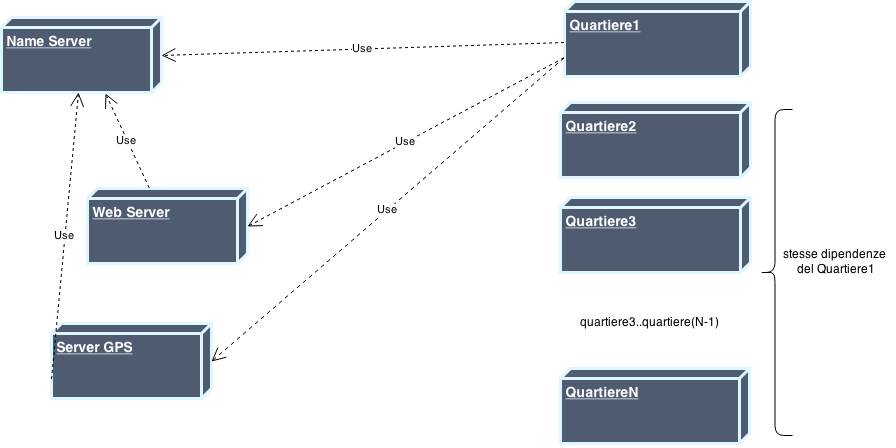
\includegraphics[width=1.0\linewidth]{DiagrammaComponenti}}
\caption{Diagramma componenti.}
\label{fig:Diagramma componenti}
\end{figure}
In questa sezione vengono descritte le componenti del sistema:
\begin{description}
\item[Quartiere:] componente che deve essere istanziata per ogni frammento della
mappa previsto dalla configurazione. Se un quartiere presenta una configurazione
valida, esso può entrare a far parte del sistema in qualunque momento (entro il
limite previsto del numero massimo di quartieri istanziabili).
Un quartiere è responsabile dello spostamento delle entità che sono in transito
in una qualunque delle strade o incroci che appartengono al quartiere stesso. Le
entità reattive quali i veicoli, le bici e i pedoni vengono istanziate in uno
specifico quartiere e le informazioni relative allo stato del percorso di queste
entità saranno sempre reperibili dal quartiere al quale l'entità è stata
istanziata, al fine di evitare che nel momento in cui un'entità debba essere
spostata da un quartiere all'altro, non occorra riportare tutto lo stato del
percorso al quartiere interessato.

Dato che, una volta configurato il sistema, le entità reattive non cambiano in
numero e contenuto informativo, conviene riportare per ogni quartiere una cache
delle entità di ogni altro quartiere al fine di evitare un numero eccessivo di
richieste a quartieri remoti responsabili dell'istanziazione delle entità
interessate durante le fase di avanzamento delle entità.
\item[Server GPS:] è una componente passiva che si occupa del calcolo del
percorso per conto di una entità. Questa componente dispone della conoscenza
della mappa di ogni quartiere correttamente istanziato. Il server GPS effettua
un aggiornamento della mappa in relazione alle nuove richieste di istanziazione
di nuovi quartieri. Il calcolo del percorso avviene eseguendo l'algoritmo di
Dijkstra dei cammini minimi. Se una certa entità deve muoversi verso una certa
destinazione non ancora raggiungibile, a causa del fatto che il quartiere
interessato non è stato ancora istanziato occorrerà ritardare lo spostamento
dell'entità. Il server per una stessa entità potrebbe calcolare percorsi minimi
diversi per 2 richieste diverse nel caso in cui nel frattempo è stato istanziato
un nuovo quartiere che presenta un percorso più breve per raggiungere la
destinazione.
\item[Web Server:] è la componente responsabile della creazione della view e
del rendering dello stato di avanzamento delle entità del sistema.
\item[Name Server:] si occupa invece di servire alle altre partizioni richieste
di accesso e riferimento a risorse che risiedono su una partizione remota.
\end{description}
\section{Strategia di avanzamento delle entità di tipo veicolo, bici o pedone}
Un primo approccio per l'avanzamento delle entità passive (veicoli, bici,
pedoni) era quello di suddividere la strada in segmenti di breve lunghezza e
permettere l'attraversamento di uno speyyone di strada ad una sola entità per
volta.
Questa strategia porta ad un avanzamento per distanze di sicurezza, ma
l'aggiornamento della nuova posizione avrebbe portato ad un avanzamento ``a
scatti'' del sistema, al di la di eventuali ottimizzazioni.

Quello che in realtà occorre considerare nell'avanzamento delle entità sono le
proprietà intrinseche del moto di avanzamento, ovvero il tempo, lo spazio,
l'accelerazione e la decelerazione. La strategia scelta segue una logica di
avanzamento secondo il modello \ac{IDM}~\cite{treiber2000microscopic}.
Seguendo il modello \ac{IDM}, l'avanzamento avviene considerando il
\textbf{\textit{delta}} di tempo nel quale il mezzo deve avanzare e le proprietà
del veicolo stesso. In relazione a questi parametri viene calcolata una
percentuale sull'accelerazione massima con cui il mezzo è stato configurato.
Infine, utilizzando il valore dell'accelerazione ottenuto, viene aggiornata la
velocità corrente e la posizione finale del mezzo.
Questi nuovi valori saranno validi alla fine del delta di tempo relativo al
periodo in cui sono stati calcolati. Di seguito vengono riportate le funzioni
matematiche utilizzate per il calcolo dello spostamento delle entità:

\begin{equation}
s^{*}(t)=s(0)+Tv(t)+\frac{v(t)\Delta{v(t)}}{2\sqrt{ab}}
\end{equation}
\begin{equation}
a(t)=a[1-(\frac{v(t)}{v_{0}})^4-(\frac{s^{*}(t)}{s(t)})^2]
\end{equation}
dove
\begin{align*}
~a =&~\text{massima accelerazione possibile}\\
v_{0} =&~ \text{elocità desiderata} \\
v(t) =&~ \text{velocità corrente} \\
s(t) =&~ \text{distanza corrente dal mezzo che sta davanti} \\
s_{0} =&~ \text{quantità minima di avanzamento} \\
s^*(t) =&~ \text{distanza calcolata in funzione dei parametri di configurazione}
\\ &~ \text{dei mezzi interessati} \\
T =&~ \text{parametro di controllo per regolamentare la velocità} \\
b =&~ \text{decelerazione massima}
\end{align*}

% $a$ è la massima accelerazione possibile; $v_{0}$ è la velocità desiderata;
% $v(t)$ è la velocità corrente; $s(t)$ è la distanza corrente dal mezzo che sta
% davanti; $s_{0}$ è la quantità minima di avanzamento; $s^*(t)$ è la distanza
% calcolata in funzione dei parametri di configurazione dei mezzi interessati; $T$
% è un altro parametro di controllo per regolamentare la velocità; $b$ è la
% decelerazione massima.

Infine è possibile aggiornare la velocità corrente della macchina e lo step di
avanzamento($ns(t)$): 

\begin{equation}
v(t)= v(t)+a\Delta
\end{equation}
\begin{equation}
ns(t)= v(t)\Delta+0.5a\Delta^2
\end{equation}

con $\Delta$ uguale al tempo desiderato per calcolare la posizione del mezzo
alla fine del $\Delta$ stesso. 

Il modello permette quindi di rappresentare una realtà continua relativa
all'avanzamento delle entità, discretizzando il tempo per una quantità $\Delta$.
In pratica, viene dato in input al modello \ac{IDM} lo stato del mezzo,
contenente la posizione corrente e i parametri di avanzamento.
Il modello ritornerà dei valori relativi all'aggiornamento della posizione delle
entità, i quali saranno validi per il modello a realtà continua alla fine
del $\Delta$ di tempo relativo al periodo in cui sono stati calcolati.

Il modello presentato richiede quindi una configurazione di alcuni parametri,
tra i quali le proprietà di moto delle entità e un parametro di sistema, ovvero
il $\Delta$. La configurazione dei parametri delle entità può essere lasciata
all'utente, predisponendo dei valori di default al fine di accelerare il
processo di configurazione delle entità.

Si è convenutio di assegnare a $\Delta$ un valore costante, quindi non
configurabile dall'utente. La scelta di tale quantità, ovvero la durata
del quanto di discretizzazione deve seguire la seguente logica:
se il $\Delta$ viene tarato con valori grandi (nell'ordine dei secondi) allora
il sistema eseguirebbe meno calcoli per completare gli spostamenti delle entità.
D'altro canto, al crescere del $\Delta$ la simulazione risulterebbe rallentata
dal punto di vista dell'avvenimento di alcuni eventi dovuti per conseguenza di
altri, ovvero le entità sarebbero poco reattive e ritarderebbero le loro azioni
in funzione della grandezza del $\Delta$. Se il $\Delta$ è troppo piccolo
(nell'ordine dei millisecondi) il sistema si troverebbe nella situazione di
eseguire molti calcoli per completare lo spostamento, le entità sarebbero
reattive, ma la quantità di avanzamento effettiva di una entità sarebbe minuta e
inutile al fine della reattività instantanea delle altre entità presenti nel
sistema. Il valore del $\Delta$ da noi scelto è \textbf{\textit{0.5 secondi}},
cosi da permettere il giusto compresso tra step di avanzamento delle entità e
reattività delle entità.
\section{Gestione del tempo tra quartieri}
Il problema principale della frammentazione della mappa in quartieri consiste nella gestione del $\Delta$ di avanzamento tra quartieri; i quartieri non possono avanzare indipendentemente l'uno dall'altro; cioè un quartiere che ha effettuato i calcoli per l'avanzamento per un certo $\Delta$, non può procedere a effettuare il calcolo di nuovi spostamenti per un nuovo $\Delta$ fino a quando tutti gli altri quartieri non hanno completato l'aggiornamento degli spostamenti delle entità al $\Delta$ precedente. Lo spostamento delle entità dei quartieri deve essere trasparente alla distribuzione della mappa, quindi un quartiere presenta una dipendenza dagli altri quartieri affinchè tutti i quartieri siano sincronizzati allo stesso quanto di tempo discretizzato. Ancora più evidente è il caso in cui un quartiere presenta un incrocio in cui per esempio una delle sue strade appartenga ad un altro quartiere; se il sistema non è sincronizzato allo stesso quanto di tempo si potrebbe incorrere nella situazione in cui un certo mezzo che debba essere spostato tra due quartieri, si trovi in attesa che il quartiere di destinazione si risincronizzi al quanto successivo; quindi avere una situazione in cui l'entità si trovi in attesa indipendentemente dalla velocità e dallo stato del traffico.\\
Dato che le entità attive del sistema sono le strade e gli incroci e la responsabilità dell'esecuzione del calcolo dell'avanzamento in un certo quanto di tempo è data sempre alle entità attive, queste dovranno rendersi partecipi nel regolamentare l'avanzamento del sistema al quanto di tempo successivo.\\

\subsection{Protocollo di sincronizzazione}
Questo protocollo si occupa di regolamentare l'avanzamento del sistema al quanto di tempo successivo; questo protocollo è quindi responsabile della gestione della logica di discretizzazione del tempo per permettere di avere una realtà continua consistente in ogni quartiere.\\
Per lo sviluppo di questo protocollo occorre considerare dapprima come il sistema viene avviato; cioè se il sistema attende che tutti i quartieri siano configurati e quindi tutti i quartieri partiranno in sincronia al tempo 0; oppure se si sceglie un approccio più flessibile in cui un quartiere viene configurato indipendentemente dagli altri e quindi entrerà in sincronizzazione in un momento non necessariamente corrispondente al tempo 0. Occorre considerare che un quartiere è una partizione a se stante, che presenta tuttavia delle dipendenze con gli altri quartieri; entrambi i sistemi di avvio presentano dei vantaggi: nel primo caso si ha che ogni quartiere aspetta che gli altri si siano configurati, si avrà quindi un ritardo nell'avvio, ma quando un quartiere ritorna dall'attesa può reperire ogni risorsa di qualunque altro quartiere dato che al ritorno dall'attesa il tutto è stato configurato; tuttavia seguendo questa idea si potrebbe presentare il caso in cui si potrebbero avere dei quartieri isolati che aspettano inutilmente altri quartieri o comunque si renderebbe impossibile la possibilità di voler aggiungere in seguito all'avvio della simulazione altri quartieri.\\
Il secondo caso invece è quello che si avvicina di più a ciò che è il paradigma della distribuzione, lasciando quindi l'indipendenza nella fase di avvio tra quartieri e quindi permettendo comunque lo spostamento di tutte le entità che presentano un percorso valido relativo al quartiere stesso, mentre per le entità che presentano delle destinazioni non raggiungibili il quartiere ne dovrà ritardare lo spostamento. Il nostro sistema implementa questa seconda scelta lasciando ove possibile l'indipendenza tra le partizioni, permettendo l'avvio del sistema e quindi dello spostamento delle entità indipendentemente dal fatto che una partizione remota sia stata configurata o meno.\\
Solo quando un quartiere presenterà richiesta di sincronizzazione allora il sistema dovrà tener conto anche della sua richiesta per permettere l'avanzamento al quanto di tempo successivo in modo da coinvolgere ogni quartiere che necessita di essere sincronizzato.\\
Tuttavia se un quartiere è stato istanziato e ha iniziato l'operazione di sincronizzazione con gli altri quartieri, in caso di fallimento o di errore durante l'esecuzione di uno qualunque di questi quartieri sincronizzati il sistema non potrà che fermarsi dato che un quartiere esegue dei servizi di spostamento per conto di entità di altri quartieri; se un quartiere da errore durante l'esecuzione lo stato del sistema diviene inconsistente e occorre riavviare il sistema e se necessario farlo ripartire dall'ultima snapshot del sistema una volta istanziati tutti i quartieri che erano stati avviati e sincronizzati all'ultima snapshot disponibile.\\
Il protocollo di sincronizzazione dovrà quindi considerare la possibilità di accogliere dei nuovi quartieri da rendere parteci alla sincronizzazione.\\
Il protocollo di sincronizzazione si divide in due parti: la sincronizzazione tra entità attive del quartiere (\ref{int_synch}) e la sincronizzazione tra quartieri (\ref{quart_synch}).
\subsubsection{Sincronizzazione tra entità attive del quartiere}
\label{int_synch}
Ogni entità attiva del quartiere dovrà comunicare ad un gestore della sincronizzazione interna del quartiere, che ha eseguito l'aggiornamento dello stato di avanzamento delle entità passive per un certo $\Delta$ di sistema. L'entità attiva dovrà poi attendere che tutto il sistema sia sincronizzato con il $\Delta$ di sistema. Solo quando l'ultima entità attiva del quartiere in questione ha eseguito l'avanzamento al $\Delta$ di sistema allora questa entità potrà avviare il protocollo di sincronizzazione tra quartieri, vedi \ref{quart_synch}.

\subsubsection{Sincronizzazione tra quartieri}
\label{quart_synch}
Il seguente protocollo è un protocollo che esegue la sincronizzazione tra un numero di quartieri non fissato a priori. Di seguito i passi del protocollo (ogni volta che appare il nome di quartiere si intenderà l'entità responsabile della sincronizzazione di tutti i quartieri allocata nel quartiere stesso):
\begin{enumerate}
\item il quartiere deve ottenere dapprima dal name server il registro dei quartieri remoti che abbiano effettuato la registrazione della mappa al server gps (da notare che quartieri distinti potrebbero ricevere risposte diverse dal nameserver, ma risposte successive saranno sempre al più un sovrainsieme delle risposte date in precedenza);
\item il quartiere (Q\_X) per ogni quartiere presente nel registro dovrà inviare una notifica testimone del fatto che Q\_X è pronto per una nuova sincronizzazione. Tale notifica potrà essere gestita dal quartiere interessato (Q\_Y) solo nel momento in cui anche Q\_Y è pronto per una nuova sincronizzazione, ovvero quando inizierà a eseguire anch'esso il protocollo (\ref{quart_synch}). L'esecuzione della procedura di notifica su Q\_Y andrà a buon fine nel caso in cui Q\_Y dispone nel proprio registro del quartiere Q\_X e in tal caso occorrerà salvare su Q\_Y il fatto che Q\_X è pronto per una nuova sincronizzazione; altrimenti Q\_Y accoda la notifica di Q\_X (lasciando in stato di attesa quindi la partizione Q\_X) al fine di poterla gestire nel quanto successivo in cui a quel punto Q\_Y certamente otterrà dal name server anche Q\_X nello step 1 del protocollo. \\
Ogni quartiere ha degli eventi che permettono di decidere il momento in cui esso può eseguire le notifiche di richiesta di nuova sincronizzazione. L'evento che permette di eseguire le procedure di notifica su Q\_Y richieste da quartieri remoti Q\_X è il passaggio dall'esecuzione di \ref{int_synch} a \ref{quart_synch} e in particolare l'esecuzione dello step 1 del protocollo. \\ La disabilitazione dell'esecuzione della procedura di notifica, operazione di \textit{CLOSE\_SYNCH}, su Q\_Y deve avvenire dall'ultimo quartiere utile che esegue su Q\_Y la procedura di notifica. Dove per ultimo quartiere utile si intende quell'ultimo quartiere (indipendentemente dall'ordine) che appartiene all'insieme minimo dei quartieri tra tutti gli insiemi di quartieri presenti nei registri dei quartieri stessi presi nello step 1 del protocollo (tale insieme d'ora in poi verrà chiamato \textit{MIN\_SET\_QUARTIERI}). \\
\item ogni quartiere presente in \textit{MIN\_SET\_QUARTIERI} dovrà quindi aspettare l'evento di chiusura della gestione delle notifiche di nuova sincronizzazione, ovvero l'evento \textit{CLOSE\_SYNCH}; a questo punto un quartiere uscente dall'attesa non conosce più lo stato di avanzamento degli altri quartieri, cioè è solo a conoscenza del fatto che tutti i quartieri in \textit{MIN\_SET\_QUARTIERI} hanno presentato nuova richiesta di sincronizzazione, ma nel frattempo uno dei quartieri in \textit{MIN\_SET\_QUARTIERI} potrebbe aver iniziato nuovamente ad eseguire il protocollo sovrascrivendo l'esecuzione delle notifiche e quindi perdendo una notifica di nuova sincronizzazione da parte di un quartiere se l'evento \textit{CLOSE\_SYNCH} non era ancora giunto. Pertanto è necessario che ogni quartiere, prima di poter eseguire nuovamente una nuova sincronizzazione, attenda l'evento \textit{CLOSE\_SYNCH} che sarà inviato da ogni altro quartiere presente in \textit{MIN\_SET\_QUARTIERI};
\end{enumerate}
Tra lo step 1 e 2 occorre integrare il seguente punto:  
\begin{itemize}
\item il quartiere deve liberare dall'attesa, se presenti, tutti quei quartieri che al $\Delta$ di sincronizzazione precedente non erano nel registro dei quartieri, supponiamo che Q\_Y nel proprio registro non contenga Q\_X, mentre Q\_X contiene nel proprio registro Q\_Y; mentre il quartiere remoto Q\_X si presta in attesa sul quartiere Q\_Y, Q\_Y non considerà Q\_X. Quindi Q\_X deve essere classificato come un quartiere nuovo che potrà entrare in sincronizzazione solo al $\Delta$ successivo; tuttavia Q\_X potrebbe nel frattempo già aver demandado l'esecuzione dello step 2 su altri quartieri che contenevano nel proprio registro Q\_X; ebbene questi quartieri dovranno ricordare tale fatto nel loro $\Delta$ di sincronizzazione successivo, dato che Q\_X a questi quartieri non invierà più la notifica di sincronizzazione; mentre Q\_Y dovrà accodare Q\_X fino alla richiesta di sincronizzazione successiva in cui appunto verrà riaccodato dallo step appena descritto nella procedura di gestione delle notifiche per il nuovo $\Delta$.
\end{itemize}

\begin{figure}[H] % Example image
\center{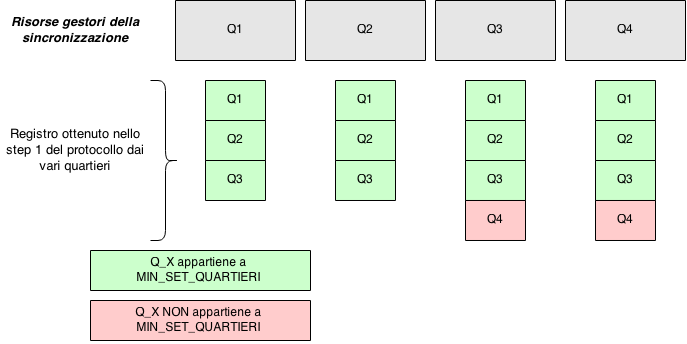
\includegraphics[width=1.0\linewidth]{ProtocolloSynch}}
\caption{Esempio di stato nella sincronizzazione dei quartieri.}
\label{fig:Esempio di stato nella sincronizzazione dei quartieri}
\end{figure}

Nell'esempio riportato i quartieri soggetti a sincronizzazione saranno Q1,Q2,Q3 mentre Q4 non potrà partecipare alla sincronizzazione, se non prima della sincronizzazione successiva in cui certamente Q1 e Q2 alla nuova richiesta del registro al name server otterranno anche Q4. Q4 cosa può fare dato che non può partecipare alla sincronizzazione? Esso potrebbe presentare una richiesta a Q1 o Q2 e in tal caso rimmarrebbe bloccato sul quartiere Q1 o Q2 dato che entrambi non dispongono di Q4; Q4 potrebbe anche presentare la richiesta a Q3 e in tal caso Q3 accoglierà Q4 e salverà temporaneamente una flag che lo avviserà per il prossimo quanto che Q4 ha già presentato richiesta di sincronizzazione. Q3 sa inoltre che non potrà attendere Q4 dato che nel momento in cui Q1 o Q2 presenteranno richiesta di sincronizzazione a Q3 invieranno anche il loro registro e li Q3 apprenderà che Q4 non è un quartiere sul quale occorre aspettare e quindi non è rilevante all'evento \textit{CLOSE\_SYNCH} nel corso del $\Delta$ corrente. Con questo semplice esempio è stato presentato un caso di sincronizzazione; ma ce ne possono essere di più complicati per esempio nel caso in cui esistesse anche un quartiere Q5 non visibile a nessuno. In tal caso alla nuova sincronizzazione Q1 Q2 e Q3 memorizzeranno nel loro registro anche Q5, mentre per Q4 il quartiere Q5 sarà un quartiere nuovo e quindi quest'ultimo potrà entrare in sincronizzazione solo al quanto successivo.

\paragraph{Considerazioni sul protocollo \ref{quart_synch}}
Questo protocollo si adatta dinamicamente a nuove richieste di sincronizzazione. Il difetto principale sta nel fatto che un quartiere dovrà attendere su altri quartieri al fine di apprendere se tutto il sistema è pronto per il passaggio al quanto successivo. In realtà l'attesa potrebbe essere rigirata sul quartiere stesso e non più sul quartiere remoto, ma data la limitazione sul numero massimo di quartieri non è un problema l'implementazione di questo protocollo anche se i quartieri utilizzano un thread-pool nella gestione delle richieste remote.

%\input{analisi_errori}
%\newpage
\appendix
\end{document}

